\chapter{Mathematical and Theoretical Background}
\label{sec:mathematical_and_theoretical_background}

This chapter presents the theoretical foundations required to understand the
methods and algorithms used throughout this thesis. In particular, it introduces
the mathematical tools needed to describe rigid body transformations and coordinate
frame relationships in robotic systems. The chapter also reviews the basic
principles of robot kinematics, camera modeling, and pose estimation techniques
used in computer vision. These concepts provide the necessary background for the
formulation and analysis of the \textit{hand-eye calibration} problem, which is
discussed in the following chapters.

% ---------------------------------------------------------------
\section{Rigid Body Transformations}
\label{sec:rigid_body}
% ---------------------------------------------------------------

In robotics and computer vision, the pose of an object or sensor in space is
commonly described through rigid body transformations \cite{craig2005introduction,
siciliano2009robotics}. A rigid body transformation represents the relative
position and orientation between two coordinate frames and consists of a rotation
and a translation. This representation is fundamental in many applications,
including robot kinematics, camera pose estimation, and calibration problems.

% -- Figure suggestion 1 --
% See image suggestion [IMG-1] at the end of this file.

\subsection{Homogeneous Transformation Matrices}
\label{subsec:homogeneous}

A rigid body transformation can be conveniently represented using
\textit{homogeneous transformation matrices}. A homogeneous transformation
combines rotation and translation into a single $4\times 4$ matrix:

\begin{equation}
    \mathbf{T} =
    \begin{bmatrix}
        \mathbf{R} & \mathbf{t} \\
        \mathbf{0}^{\top} & 1
    \end{bmatrix}
    \in SE(3)
    \label{eq:homogeneous_transform}
\end{equation}

\noindent where $\mathbf{R} \in \mathbb{R}^{3 \times 3}$ is a rotation matrix
describing the orientation between the two frames, and $\mathbf{t} \in
\mathbb{R}^3$ is a translation vector representing their relative position.

Using this formulation, a point $\mathbf{p}$ expressed in one coordinate frame
can be transformed into another frame through matrix multiplication. Given a
point ${}^B\mathbf{p}$ expressed in frame $\{B\}$, its coordinates in frame
$\{A\}$ are obtained as:

\begin{equation}
    \begin{bmatrix} {}^A\mathbf{p} \\ 1 \end{bmatrix}
    = {}^A_B\mathbf{T}
    \begin{bmatrix} {}^B\mathbf{p} \\ 1 \end{bmatrix}
    =
    \begin{bmatrix} {}^A_B\mathbf{R} & {}^A\mathbf{t}_{B} \\
    \mathbf{0}^{\top} & 1 \end{bmatrix}
    \begin{bmatrix} {}^B\mathbf{p} \\ 1 \end{bmatrix}
    \label{eq:point_transform}
\end{equation}







\begin{figure}[htbp]
	\centering
	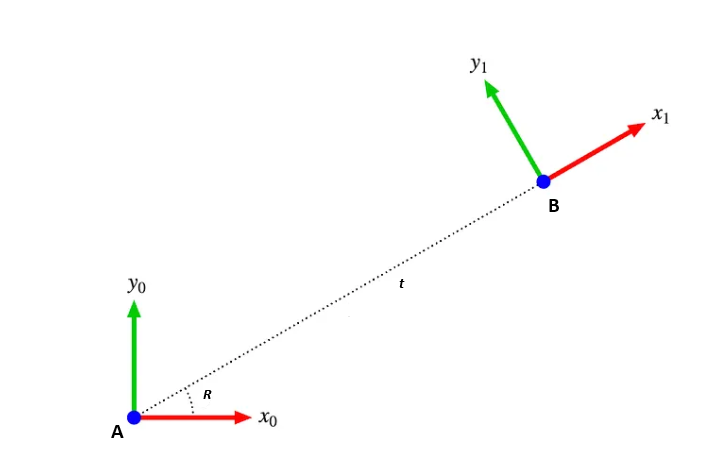
\includegraphics[width=0.6\textwidth]{images/chapter2Images/frame2frame.png}
	\caption{Rigid body transformation between two coordinate frames. 
		The pose of frame $\{B\}$ with respect to frame $\{A\}$ is described 
		by a rotation $\mathbf{R}$ and a translation $\mathbf{t}$, combined 
		in the homogeneous transformation matrix ${}^A_B\mathbf{T} \in SE(3)$.}
	\label{fig:frame_to_frame}
\end{figure}

As illustrated in Figure~\ref{fig:frame_to_frame}, a rigid body transformation
encodes both the relative orientation and position between two coordinate frames.


\noindent Homogeneous transformations also allow multiple transformations to be
composed by multiplying the corresponding matrices, which is particularly useful
when dealing with chains of coordinate transformations in robotic systems
\cite{craig2005introduction}:

\begin{equation}
    {}^A_C\mathbf{T} = {}^A_B\mathbf{T} \cdot {}^B_C\mathbf{T}
    \label{eq:chain}
\end{equation}

The inverse of a homogeneous transformation is given by:

\begin{equation}
    \mathbf{T}^{-1} =
    \begin{bmatrix}
        \mathbf{R}^{\top} & -\mathbf{R}^{\top}\mathbf{t} \\
        \mathbf{0}^{\top} & 1
    \end{bmatrix}
    \label{eq:T_inverse}
\end{equation}

\noindent which follows directly from the properties of rotation matrices
($\mathbf{R}^{-1} = \mathbf{R}^{\top}$, since $\mathbf{R} \in SO(3)$).

\subsection{Rotation Representations}
\label{subsec:rotations}

The rotational component of a rigid transformation can be represented in several
ways, each with different properties in terms of compactness, singularities, and
computational efficiency \cite{siciliano2009robotics, murray1994mathematical}.

% -- Figure suggestion 2 --
% See image suggestion [IMG-2] at the end of this file.

\paragraph{Rotation Matrix.}
A rotation matrix $\mathbf{R} \in SO(3)$ is a $3\times3$ orthogonal matrix with
determinant equal to $+1$:

\begin{equation}
    SO(3) = \left\{ \mathbf{R} \in \mathbb{R}^{3\times3} \;\middle|\;
    \mathbf{R}^{\top}\mathbf{R} = \mathbf{I},\; \det(\mathbf{R}) = +1 \right\}
    \label{eq:SO3}
\end{equation}

\noindent A rotation matrix has nine entries but only three independent degrees
of freedom, and it can be constructed as the product of three elementary
rotations around the coordinate axes.



\paragraph{Euler Angles.}
Euler angles describe a rotation as a sequence of three rotations around
coordinate axes, parameterized by three angles $(\alpha, \beta, \gamma)$.
For example, the ZYX convention (roll--pitch--yaw) commonly used in robotics
composes the rotation as:

\begin{equation}
    \mathbf{R}_{ZYX}(\alpha,\beta,\gamma) =
    \mathbf{R}_z(\alpha)\,\mathbf{R}_y(\beta)\,\mathbf{R}_x(\gamma)
    \label{eq:euler}
\end{equation}

\noindent While intuitive, Euler angles suffer from a representation singularity
known as \textit{gimbal lock}, which occurs when two of the rotation axes become
aligned, causing a loss of one degree of freedom \cite{craig2005introduction}.

\paragraph{Axis--Angle and Rodrigues Vector.}
The axis--angle representation defines a rotation by a unit vector
$\hat{\mathbf{k}} \in \mathbb{R}^3$ (the rotation axis) and a scalar $\theta$
(the rotation angle). The corresponding rotation matrix is given by
Rodrigues' rotation formula:

\begin{equation}
    \mathbf{R} = \mathbf{I} + \sin\theta\,[\hat{\mathbf{k}}]_{\times}
    + (1 - \cos\theta)\,[\hat{\mathbf{k}}]_{\times}^2
    \label{eq:rodrigues}
\end{equation}

\noindent where $[\hat{\mathbf{k}}]_{\times}$ denotes the skew-symmetric matrix
associated with $\hat{\mathbf{k}}$:

\begin{equation}
    [\hat{\mathbf{k}}]_{\times} =
    \begin{bmatrix}
        0 & -k_z & k_y \\
        k_z & 0 & -k_x \\
        -k_y & k_x & 0
    \end{bmatrix}
    \label{eq:skew}
\end{equation}

\noindent The \textit{Rodrigues vector} $\mathbf{r} = \theta\hat{\mathbf{k}}$
provides a compact three-parameter representation widely used in computer vision
libraries such as OpenCV \cite{bradski2008learning}.

\paragraph{Quaternions.}
A unit quaternion $\mathbf{q} = (q_w, q_x, q_y, q_z)$ with
$q_w^2 + q_x^2 + q_y^2 + q_z^2 = 1$ provides another representation of
rotations. Its relation to the axis--angle parameterization is:

\begin{equation}
    \mathbf{q} = \left(\cos\frac{\theta}{2},\;
    \hat{\mathbf{k}}\sin\frac{\theta}{2}\right)
    \label{eq:quaternion}
\end{equation}

\noindent Quaternions avoid gimbal lock, provide good numerical stability, and
support efficient interpolation via \textit{SLERP} (Spherical Linear
intERPolation), making them particularly useful in optimization and control
contexts \cite{daniilidis1999hand}.

\subsection{Lie Groups \texorpdfstring{$SO(3)$}{SO(3)} and
\texorpdfstring{$SE(3)$}{SE(3)}}
\label{subsec:lie}

From a mathematical perspective, rotations and rigid body transformations can
be described using the framework of \textit{Lie groups}
\cite{murray1994mathematical}. The set of all three-dimensional rotation matrices
forms the special orthogonal group $SO(3)$, while the set of rigid body
transformations forms the special Euclidean group:

\begin{equation}
    SE(3) = \left\{
    \begin{bmatrix} \mathbf{R} & \mathbf{t} \\ \mathbf{0}^{\top} & 1
    \end{bmatrix}
    \;\middle|\; \mathbf{R} \in SO(3),\; \mathbf{t} \in \mathbb{R}^3
    \right\}
    \label{eq:SE3}
\end{equation}

\noindent Each Lie group has an associated \textit{Lie algebra}, which provides
a local linearization of the group around the identity. For $SO(3)$, the
corresponding Lie algebra $\mathfrak{so}(3)$ consists of $3\times3$
skew-symmetric matrices; for $SE(3)$, the Lie algebra $\mathfrak{se}(3)$
consists of $4\times4$ matrices of the form:

\begin{equation}
    \hat{\xi} =
    \begin{bmatrix} [\boldsymbol{\omega}]_{\times} & \mathbf{v} \\
    \mathbf{0}^{\top} & 0 \end{bmatrix}
    \in \mathfrak{se}(3)
    \label{eq:se3_algebra}
\end{equation}

\noindent where $\boldsymbol{\omega} \in \mathbb{R}^3$ represents the angular
velocity and $\mathbf{v} \in \mathbb{R}^3$ represents the linear velocity.
The vector $\xi = (\boldsymbol{\omega}, \mathbf{v}) \in \mathbb{R}^6$ is called
a \textit{twist}. \cite{murray1994mathematical}  The exponential map $\exp: \mathfrak{se}(3) \to SE(3)$ allows
elements of the Lie algebra to be mapped back to the group, and is the basis for
the \textit{product of exponentials} formulation of robot kinematics
\cite{murray1994mathematical}. This Lie group formalism provides the theoretical
foundation for the hand-eye calibration algorithms discussed in
Chapter~\ref{sec:problem_statement}.

% ---------------------------------------------------------------
\section{Robot Kinematics}
\label{sec:robot_kinematics}
% ---------------------------------------------------------------

Robot kinematics is the study of the geometric relationships between the links
and joints of a robotic manipulator, without considering the forces that cause
motion \cite{siciliano2009robotics, craig2005introduction}. In the context of
this work, an understanding of forward kinematics is essential since the robot
end-effector poses recorded during the calibration procedure are computed from
the robot joint readings.

\subsection{Robot Structure and Joint Space}
\label{subsec:robot_structure}

A serial robotic manipulator consists of a sequence of rigid \textit{links}
connected by \textit{joints}. Each joint provides one degree of freedom:
\textit{revolute} joints allow rotation about an axis, while
\textit{prismatic} joints allow translation along an axis. A manipulator with
$n$ joints has a joint space $\mathcal{Q} \subset \mathbb{R}^n$, where the
configuration is described by the joint variable vector:

\begin{equation}
    \mathbf{q} = \begin{bmatrix} q_1 & q_2 & \cdots & q_n \end{bmatrix}^{\top}
    \in \mathcal{Q}
    \label{eq:joint_vector}
\end{equation}

\noindent where $q_i$ is the $i$-th joint angle (for revolute joints) or
displacement (for prismatic joints).

% -- Figure suggestion 3 --
% See image suggestion [IMG-3] at the end of this file.

\subsection{Denavit--Hartenberg Convention}
\label{subsec:dh}

A systematic method for assigning coordinate frames to the links of a serial
manipulator is given by the \textit{Denavit--Hartenberg (DH) convention},
introduced in \cite{denavit1955kinematic}. According to this convention, a
coordinate frame $\{i\}$ is attached to each link $i$, and the transformation
from frame $\{i-1\}$ to frame $\{i\}$ is described by exactly four parameters:

\begin{itemize}
    \item $a_i$: the \textit{link length}, i.e.\ the distance between axes
    $z_{i-1}$ and $z_i$ measured along $x_i$.
    \item $\alpha_i$: the \textit{link twist}, i.e.\ the angle between axes
    $z_{i-1}$ and $z_i$ measured about $x_i$.
    \item $d_i$: the \textit{link offset}, i.e.\ the distance between axes
    $x_{i-1}$ and $x_i$ measured along $z_{i-1}$.
    \item $\theta_i$: the \textit{joint angle}, i.e.\ the angle between axes
    $x_{i-1}$ and $x_i$ measured about $z_{i-1}$.
\end{itemize}


\begin{figure}[htbp]
	\centering
	
	\begin{subfigure}{0.48\textwidth}
		\centering
		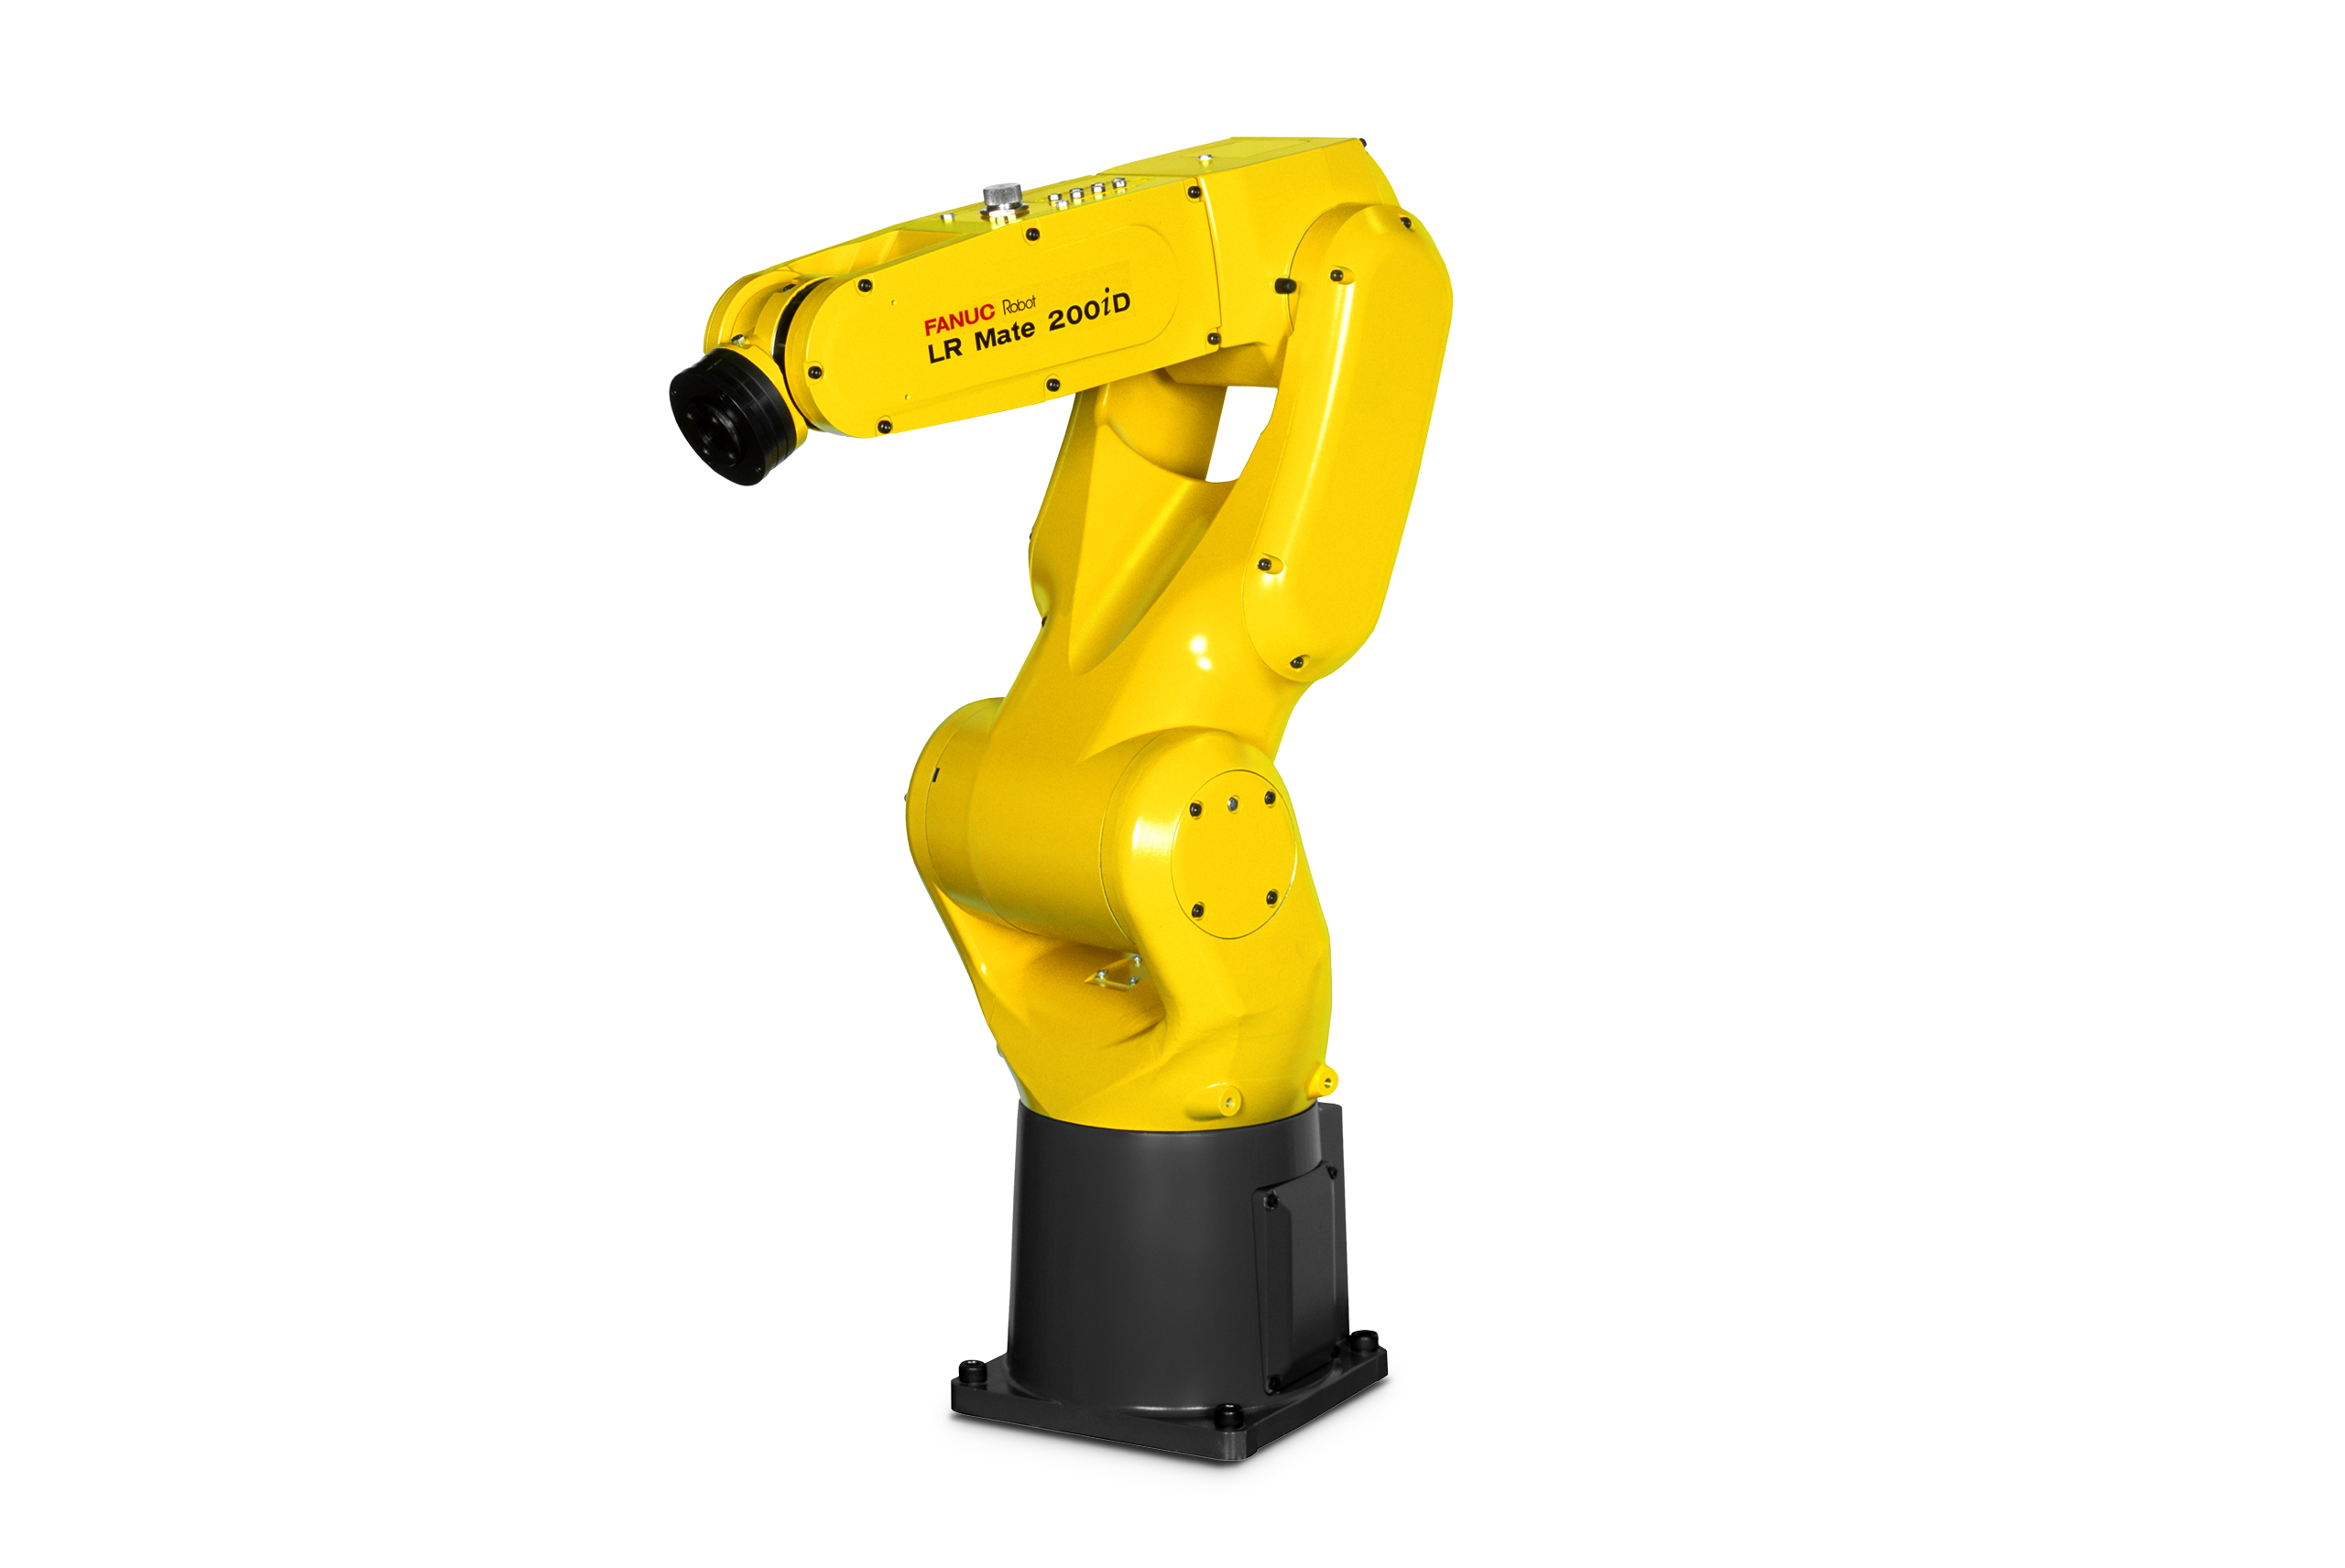
\includegraphics[width=\linewidth]{images/chapter2Images/FanucLRMate200id.png}
		\caption{Industrial robotic manipulator (example platform).}
		\label{fig:fanuc_robot}
	\end{subfigure}
	\hfill
	\begin{subfigure}{0.48\textwidth}
		\centering
		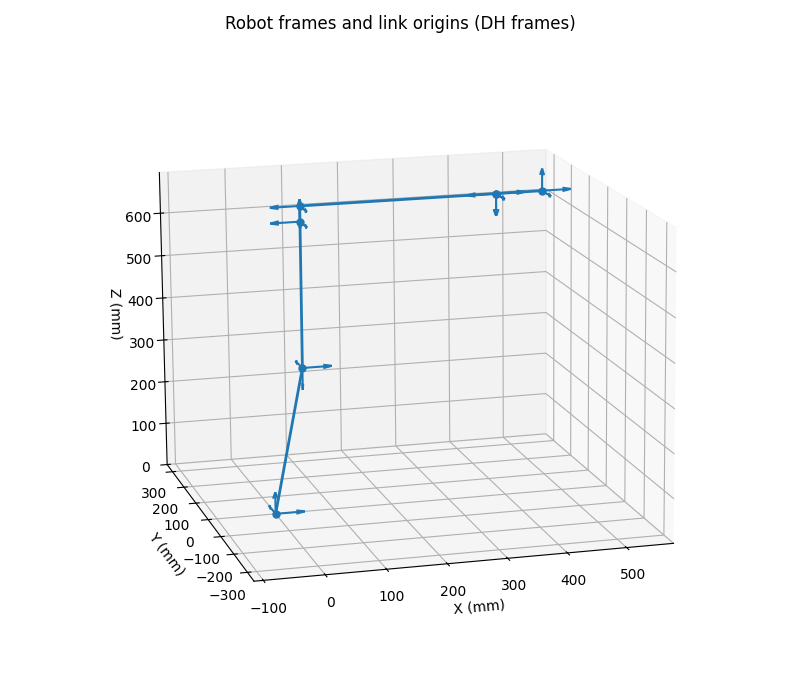
\includegraphics[width=\linewidth]{images/chapter2Images/denavitHartenberg.png}
		\caption{Assignment of coordinate frames using the Denavit--Hartenberg convention.}
		\label{fig:dh_frames}
	\end{subfigure}
	
	\caption{Robot kinematic structure and coordinate frame assignment.}
	\label{fig:robot_kinematics}
\end{figure}

As shown in Figure~\ref{fig:robot_kinematics}, a robotic manipulator can be modeled
as a sequence of rigid links, each associated with a coordinate frame
according to the Denavit--Hartenberg convention.

The homogeneous transformation matrix from frame $\{i-1\}$ to frame $\{i\}$
is then given by the product of four elementary transformations:

\begin{equation}
    {}^{i-1}_{i}\mathbf{T}(\theta_i) =
    \mathbf{R}_z(\theta_i)\, \mathbf{T}_z(d_i)\,
    \mathbf{T}_x(a_i)\, \mathbf{R}_x(\alpha_i)
    \label{eq:dh_product}
\end{equation}

\noindent which expands to:

\begin{equation}
    {}^{i-1}_{i}\mathbf{T} =
    \begin{bmatrix}
        \cos\theta_i & -\sin\theta_i\cos\alpha_i &  \sin\theta_i\sin\alpha_i & a_i\cos\theta_i \\
        \sin\theta_i &  \cos\theta_i\cos\alpha_i & -\cos\theta_i\sin\alpha_i & a_i\sin\theta_i \\
        0            &  \sin\alpha_i             &  \cos\alpha_i             & d_i             \\
        0            &  0                        &  0                        & 1
    \end{bmatrix}
    \label{eq:dh_matrix}
\end{equation}

% -- Figure suggestion 4 --
% See image suggestion [IMG-4] at the end of this file.

\subsection{Forward Kinematics}
\label{subsec:fk}

\textit{Forward kinematics} refers to the problem of computing the pose of the
robot end-effector in the base frame given a set of joint values
$\mathbf{q}$ \cite{craig2005introduction, siciliano2009robotics}. For a
serial manipulator with $n$ joints, the end-effector transformation with respect
to the base frame is obtained by composing all the DH link transformations:

\begin{equation}
    {}^0_n\mathbf{T}(\mathbf{q}) =
    {}^0_1\mathbf{T}(q_1)\cdot
    {}^1_2\mathbf{T}(q_2) \cdots
    {}^{n-1}_n\mathbf{T}(q_n)
    = \prod_{i=1}^{n} {}^{i-1}_i\mathbf{T}(q_i)
    \label{eq:fk}
\end{equation}

\noindent The result ${}^0_n\mathbf{T} \in SE(3)$ encodes the full pose
(position and orientation) of the end-effector in the robot base frame and
is the quantity directly used in the hand-eye calibration procedure.

In practice, the robot controller provides the end-effector pose directly
from encoder readings via the robot's built-in forward kinematics solver.
These poses are recorded during the calibration data acquisition phase and
correspond to the matrices $\mathbf{A}_i$ in the calibration
equation~\eqref{eq:axb}.









% ---------------------------------------------------------------
\section{Camera Model}
\label{sec:camera_model}
% ---------------------------------------------------------------

In computer vision systems, the camera model describes how three-dimensional
points in the physical world are projected onto a two-dimensional image plane
\cite{hartley2004multiple}. A mathematical model of the camera is necessary to
interpret image measurements and to estimate the spatial relationship between
the camera and objects in the environment. Camera models are therefore a
fundamental component in tasks such as pose estimation, camera calibration, and
vision-guided robotics \cite{bradski2008learning}.

\subsection{Pinhole Camera Model}
\label{subsec:pinhole}

The most widely used camera model in computer vision is the
\textit{pinhole camera model} \cite{hartley2004multiple}. This model approximates
the image formation process by assuming that all light rays pass through a single
point called the \textit{optical center} (or projection center) before hitting the
image plane. Let a point ${}^C\mathbf{P} = (X, Y, Z)^{\top}$ be expressed in the
camera coordinate frame, with $Z > 0$. The perspective projection onto the image
plane at distance $f$ (the focal length) is described by:

\begin{equation}
    x = f \frac{X}{Z}, \qquad y = f \frac{Y}{Z}
    \label{eq:perspective_proj}
\end{equation}


\begin{figure}[htbp]
	\centering
	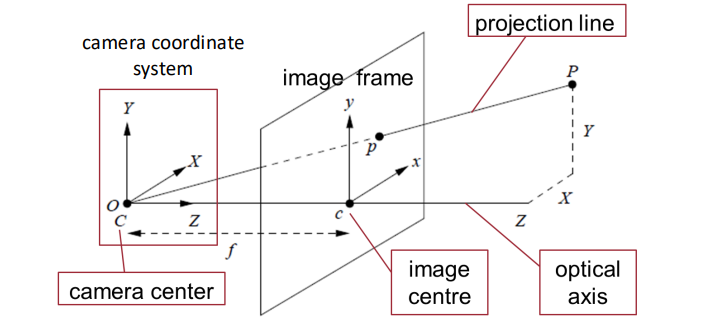
\includegraphics[width=0.75\textwidth]{images/chapter2Images/pinholeCameraModel.png}
	\caption{Pinhole camera model. A 3D point $\mathbf{P}(X,Y,Z)$ is projected through the optical center onto the image plane, generating the image point $\mathbf{p}(x,y)$.}
	\label{fig:pinhole_camera_model}
\end{figure}

As illustrated in Figure~\ref{fig:pinhole_camera_model}, the image formation
process can be interpreted geometrically as the intersection between the image
plane and the projection ray connecting the 3D point to the optical center.

\noindent where $(x, y)$ are the coordinates of the projected point in the
\textit{normalized image plane}. This transformation is non-linear due to the
division by $Z$, but it can be made linear by using homogeneous coordinates.




% -- Figure [IMG-5]: Pinhole projection diagram --
% (see figure suggestions at the end of this section)

\subsection{Intrinsic Parameters and Camera Matrix}
\label{subsec:intrinsics}

In practice, image coordinates are expressed in pixels rather than metric units,
and the principal point (the projection of the optical center onto the image plane)
is generally not at the pixel-coordinate origin. These effects are captured by the
\textit{intrinsic parameters} of the camera, collected in the $3 \times 3$ camera
matrix $\mathbf{K}$:

\begin{equation}
    \mathbf{K} =
    \begin{bmatrix}
        f_x & s   & c_x \\
        0   & f_y & c_y \\
        0   & 0   & 1
    \end{bmatrix}
    \label{eq:camera_matrix}
\end{equation}

\noindent where $f_x$ and $f_y$ are the focal lengths expressed in pixel units
along the $x$ and $y$ axes respectively, $(c_x, c_y)$ is the
\textit{principal point}, and $s$ is the skew coefficient (typically zero for
modern cameras). These parameters are determined through a camera calibration
procedure \cite{zhang2000flexible}. When a non-zero skew is present, the pixel
axes are not perpendicular; in practice $s \approx 0$ is a standard assumption.

\subsection{Fisheye Camera Model}
\label{subsec:fisheye}

In some applications, cameras with a very wide field of view (up to or beyond
$180^{\circ}$) are used in order to capture a larger portion of the environment.
These cameras employ fisheye lenses, which obey a fundamentally different
projection law than the standard pinhole model. Specifically, the relationship
between the angle of incidence $\theta$ (measured from the optical axis) and
the radial distance $r$ from the principal point in the image is not the
perspective law $r = f\tan\theta$ but instead approximates:

\begin{equation}
    r(\theta) = k_1\theta + k_3\theta^3 + k_5\theta^5 + k_7\theta^7 + k_9\theta^9
    \label{eq:fisheye_proj}
\end{equation}

\noindent where $k_1, k_3, k_5, k_7, k_9$ are model parameters estimated
during calibration \cite{kannala2006generic}. This \textit{equidistant-based
generic model} (Kannala--Brandt model) is suitable for fish-eye lenses as well
as conventional and wide-angle cameras, and is widely used in robotics and SLAM
applications.

\subsection{Lens Distortion}
\label{subsec:distortion}

Real lenses introduce geometric distortions that cause deviations from the ideal
pinhole model \cite{hartley2004multiple, bradski2008learning}. The two dominant
types are:

\paragraph{Radial distortion.} Points are displaced radially from the principal
point. The corrected normalized coordinates $(x_c, y_c)$ are related to the
distorted coordinates $(x_d, y_d)$ by:

\begin{equation}
    x_c = x_d (1 + k_1 r^2 + k_2 r^4 + k_3 r^6), \quad
    y_c = y_d (1 + k_1 r^2 + k_2 r^4 + k_3 r^6)
    \label{eq:radial_distortion}
\end{equation}

\noindent where $r^2 = x_d^2 + y_d^2$ and $k_1, k_2, k_3$ are the radial
distortion coefficients.

\paragraph{Tangential distortion.} Caused by slight misalignment between the
lens and the image sensor:

\begin{equation}
    \begin{aligned}
    x_c &= x_d + \bigl[2p_1 x_d y_d + p_2(r^2 + 2x_d^2)\bigr] \\
    y_c &= y_d + \bigl[p_1(r^2 + 2y_d^2) + 2p_2 x_d y_d\bigr]
    \end{aligned}
    \label{eq:tangential_distortion}
\end{equation}

\noindent where $p_1$ and $p_2$ are the tangential distortion coefficients.
The full distortion vector used by OpenCV is therefore
$(k_1, k_2, p_1, p_2, k_3)$ \cite{bradski2008learning}.

\begin{figure}[htbp]
	\centering
	
	\begin{subfigure}{\linewidth}
		\centering
		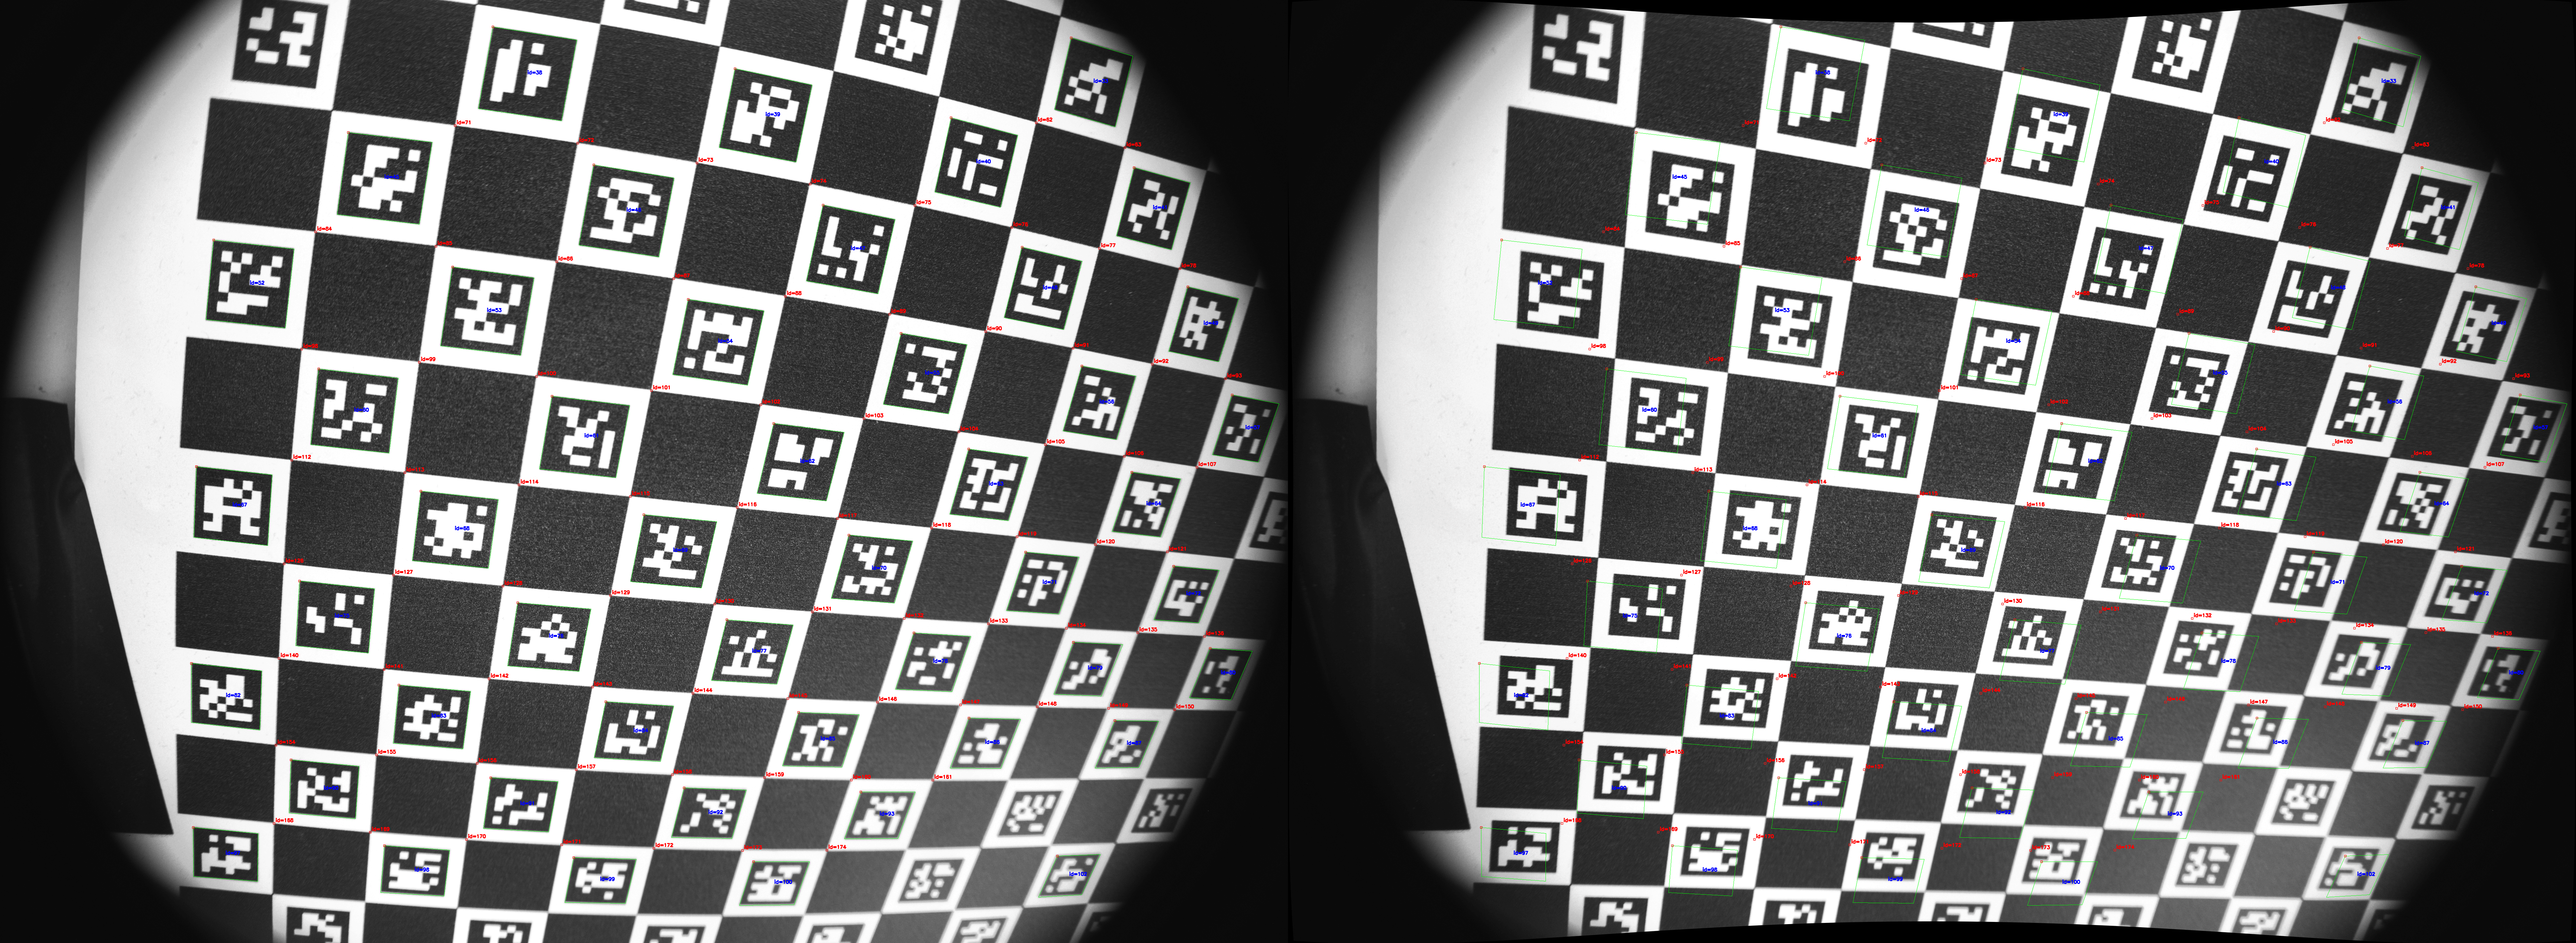
\includegraphics[width=\linewidth]{images/chapter2Images/005_comparison_markers.png}
		\caption{Effect of lens distortion on ChArUco marker detection.}
		\label{fig:lens_distortion_comparison}
	\end{subfigure}
	
	\vspace{0.5cm}
	
	\begin{subfigure}{\linewidth}
		\centering
		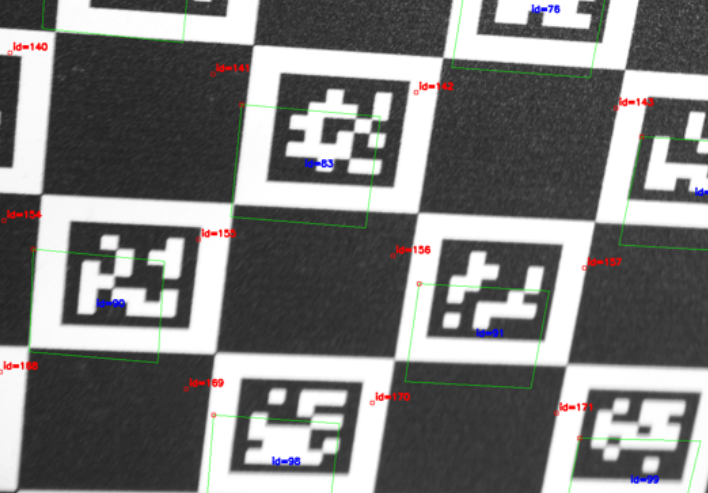
\includegraphics[width=\linewidth]{images/chapter2Images/005_comparison_markers_zoom.png}
		\caption{Zoomed-in region highlighting marker displacement.}
		\label{fig:distortion_zoom}
	\end{subfigure}
	
	\caption{Impact of lens distortion on ChArUco corner localization.
		The distortion causes systematic displacement of image features,
		which can negatively affect pose estimation and calibration accuracy.}
	\label{fig:distortion_full}
\end{figure}

% -- Figure [IMG-6]: Radial distortion effect --
% (see figure suggestions at the end of this section)




\subsection{Full Projection Equation}
\label{subsec:projection_eq}

Combining the camera intrinsics, the distortion model, and the camera pose
with respect to the world frame, the projection of a 3D world point
${}^W\mathbf{P} \in \mathbb{R}^3$ onto the image plane can be written in
homogeneous coordinates as:

\begin{equation}
    s \, \tilde{\mathbf{p}} = \mathbf{K}
    \begin{bmatrix} \mathbf{R} \mid \mathbf{t} \end{bmatrix}
    \widetilde{{}^W\mathbf{P}}
    \label{eq:projection}
\end{equation}

\noindent where $s$ is a scalar scale factor, $\tilde{\mathbf{p}} =
(u, v, 1)^{\top}$ are the homogeneous image coordinates in pixels,
$\widetilde{{}^W\mathbf{P}} = (X_W, Y_W, Z_W, 1)^{\top}$ are homogeneous world
coordinates, $[\mathbf{R} \mid \mathbf{t}]$ is the $3 \times 4$ extrinsic matrix
describing the camera pose with respect to the world frame, and $\mathbf{K}$ is
the intrinsic matrix from~\eqref{eq:camera_matrix}. This equation forms the basis
of most geometric computer vision algorithms, including pose estimation methods
used in hand-eye calibration.




% ---------------------------------------------------------------
\section{Pose Estimation}
\label{sec:pose_estimation}
% ---------------------------------------------------------------

Pose estimation is a fundamental problem in computer vision, consisting in
determining the position and orientation of a camera with respect to a known
reference object \cite{hartley2004multiple}. In the context of vision-guided
robotic systems, pose estimation is typically performed by observing a calibration
target — such as a checkerboard or fiducial marker board — and computing the
rigid transformation between the camera and the target reference frame. This step
provides the camera motion information required for hand-eye calibration.

\subsection{The Perspective-\textit{n}-Point Problem}
\label{subsec:pnp}

The pose estimation problem is commonly formulated as the
\textit{Perspective-$n$-Point} (P$n$P) problem \cite{lepetit2009epnp}. Given:
\begin{itemize}
    \item a set of $n$ known 3D points $\{\mathbf{P}_i\}_{i=1}^{n}$ expressed in
    a reference (object) coordinate frame,
    \item their corresponding 2D projections $\{\mathbf{p}_i\}_{i=1}^{n}$
    detected in the image,
    \item the camera intrinsic matrix $\mathbf{K}$ and distortion coefficients,
\end{itemize}

\noindent the goal is to estimate the rotation $\mathbf{R}$ and translation
$\mathbf{t}$ such that the reprojection equation~\eqref{eq:projection} is
satisfied for all $i$. Formally, the P$n$P problem seeks:


\begin{equation}
	(\mathbf{R}^*, \mathbf{t}^*) =
	\arg\min_{\mathbf{R} \in SO(3),\, \mathbf{t} \in \mathbb{R}^3}
	\sum_{i=1}^{n}
	\left\|
	\mathbf{p}_i -
	\pi\!\left(\mathbf{K},\, \mathbf{R},\, \mathbf{t},\, \mathbf{P}_i\right)
	\right\|^2
	\label{eq:pnp_reprojection}
\end{equation}

\noindent where $\pi(\cdot)$ denotes the projection function defined in
equation~\eqref{eq:projection}. This quantity is known as the
\textit{reprojection error} and is the standard metric for evaluating pose
estimation accuracy.

The estimated pose is obtained by minimizing the discrepancy
between the observed image points and the projections of the
corresponding 3D points onto the image plane.
Several algorithms have been proposed to solve the P$n$P problem. Classical
methods such as the Direct Linear Transform (DLT) require at least $n = 6$
point correspondences and solve a linear system \cite{hartley2004multiple}.
More efficient methods, such as the \textit{EPnP} algorithm proposed by Lepetit
et al.\ \cite{lepetit2009epnp}, provide an accurate non-iterative solution in
$O(n)$ time for $n \geq 4$ by expressing the $n$ 3D points as weighted sums
of four virtual control points, reducing the problem to a small eigenvalue
system. In practice, a larger number of points is used to improve robustness
against detection noise.

\subsection{Pose Estimation with OpenCV}
\label{subsec:pnp_opencv}

In practical implementations, pose estimation is commonly performed using the
\texttt{cv::solvePnP()} function from the OpenCV library
\cite{bradski2008learning}. Its main inputs are:
\begin{itemize}
    \item the 3D object points $\{\mathbf{P}_i\}$ in the object frame,
    \item the corresponding 2D image points $\{\mathbf{p}_i\}$ detected in
    the image,
    \item the camera intrinsic matrix $\mathbf{K}$,
    \item the distortion coefficient vector $(k_1, k_2, p_1, p_2, k_3)$.
\end{itemize}

\noindent The function returns the estimated pose as a Rodrigues rotation vector
$\mathbf{r} = \theta\hat{\mathbf{k}}$ (see Section~\ref{subsec:rotations}) and a
translation vector $\mathbf{t}$, which can be composed into the homogeneous
transformation matrix:

\begin{equation}
    {}^C_O\mathbf{T} =
    \begin{bmatrix}
        \mathbf{R}(\mathbf{r}) & \mathbf{t} \\
        \mathbf{0}^{\top} & 1
    \end{bmatrix} \in SE(3)
    \label{eq:pnp_output}
\end{equation}

\noindent where ${}^C_O\mathbf{T}$ represents the pose of the calibration target
(object frame $O$) with respect to the camera frame $C$. Several solver methods
are available through the \texttt{flags} argument, including \texttt{SOLVEPNP\_EPNP}
\cite{lepetit2009epnp} and \texttt{SOLVEPNP\_ITERATIVE} (a Levenberg--Marquardt
refinement). In this work, the output transformation ${}^C_O\mathbf{T}$ directly
provides the camera motion $\mathbf{B}_i$ used in the calibration
equation~\eqref{eq:axb}.

\subsection{Planar and Non-Planar Configurations}
\label{subsec:planar}

The geometric distribution of the 3D reference points significantly affects the
stability and accuracy of the P$n$P solution \cite{hartley2004multiple}.

\paragraph{Planar configurations.} When all reference points lie on a single plane
(as is the case with checkerboard targets and flat marker boards), the pose
estimation problem can be treated as a \textit{homography estimation} problem.
Specialized planar P$n$P solvers exploit the planarity constraint to reduce the
degrees of freedom, but planar configurations can lead to a two-fold pose ambiguity
when the target is nearly fronto-parallel to the camera \cite{zhang2000flexible}.

\paragraph{Non-planar configurations.} Points distributed in 3D space provide
stronger geometric constraints and yield more stable pose estimates. However,
3D calibration targets are more complex to manufacture and use in practice.

In many hand-eye calibration setups, planar targets such as checkerboards are
preferred due to their simplicity and ease of use \cite{zhang2000flexible,
enebuse2021comparative}. The transformation ${}^C_O\mathbf{T}$ estimated at each
robot pose constitutes the camera motion measurement $\mathbf{B}_i$ in
equation~\eqref{eq:axb}.

\bigskip
\noindent\textit{Suggested figure for this section:}
\begin{itemize}
    \item \textbf{[IMG-7]} A checkerboard image with the detected corners
    overlaid as colored dots and the estimated coordinate axes (RGB = XYZ)
    drawn at the board origin. This can be generated directly from OpenCV's
    \texttt{cv::drawChessboardCorners()} and
    \texttt{cv::drawFrameAxes()} functions on one of your own calibration
    images. It is the single most effective figure for this section.
\end{itemize}




% ---------------------------------------------------------------
\section{Hand-Eye Calibration Theory}
\label{sec:hec_theory}
% ---------------------------------------------------------------

Hand-eye calibration is a fundamental problem in vision-guided robotic systems,
consisting in determining the rigid transformation between a camera and a robot.
This transformation allows measurements obtained from the vision system to be
correctly interpreted within the robot coordinate frame. The theoretical concepts
introduced in the previous sections — rigid body transformations, robot
kinematics, and pose estimation — provide the necessary tools to formulate and
solve this problem \cite{shiu1989calibration, tsai1989new, horaud1995hand}.

% ---------------------------------------------------------------
\subsection{Problem Formulation}
\label{subsec:hec_formulation}
% ---------------------------------------------------------------

Consider a robot manipulator that is moved through a sequence of $n$ poses while
a calibration target is observed by a camera. At each step $i$, two relative
motions can be measured independently:

\begin{itemize}
    \item $\mathbf{A}_i \in SE(3)$: the relative motion of the robot end-effector
    between pose $i$ and a reference pose, obtained directly from the robot's
    forward kinematics (Section~\ref{subsec:fk}).
    \item $\mathbf{B}_i \in SE(3)$: the corresponding relative motion of the
    calibration target as seen by the camera, obtained from pose estimation
    (Section~\ref{sec:pose_estimation}).
\end{itemize}

If a rigid, fixed transformation $\mathbf{X} \in SE(3)$ relates the camera frame
to the robot end-effector frame, then for every pair of poses the following
constraint must hold simultaneously:

\begin{equation}
    \mathbf{A}_i \mathbf{X} = \mathbf{X} \mathbf{B}_i,
    \qquad i = 1, \dots, n
    \label{eq:axxb}
\end{equation}

\noindent This is the classical hand-eye calibration equation, first formulated
by Shiu and Ahmad \cite{shiu1989calibration} and independently by Tsai and Lenz
\cite{tsai1989new}. The unknown $\mathbf{X}$ is the transformation to be
estimated from the set of motion pairs $\{(\mathbf{A}_i, \mathbf{B}_i)\}$.

Decomposing equation~\eqref{eq:axxb} into its rotational and translational
components (using the notation $\mathbf{A}_i = (\mathbf{R}_{A_i}, \mathbf{t}_{A_i})$
and $\mathbf{X} = (\mathbf{R}_X, \mathbf{t}_X)$) yields two coupled sub-problems:

\begin{align}
    \mathbf{R}_{A_i} \mathbf{R}_X &= \mathbf{R}_X \mathbf{R}_{B_i}
    \label{eq:rot_subproblem} \\
    \mathbf{R}_{A_i} \mathbf{t}_X + \mathbf{t}_{A_i}
    &= \mathbf{R}_X \mathbf{t}_{B_i} + \mathbf{t}_X
    \label{eq:trans_subproblem}
\end{align}

\noindent Equation~\eqref{eq:rot_subproblem} depends only on $\mathbf{R}_X$ and
can be solved first. Once $\mathbf{R}_X$ is known, equation~\eqref{eq:trans_subproblem}
becomes a linear system in $\mathbf{t}_X$. This two-stage strategy is the basis
of classical methods such as Tsai--Lenz \cite{tsai1989new} and Horaud--Dornaika
\cite{horaud1995hand}. More recent approaches, including the dual quaternion method
of Daniilidis \cite{daniilidis1999hand} and the Lie group formulation of Park and
Martin \cite{park1994robot}, solve for rotation and translation simultaneously,
which generally leads to better robustness in the presence of noise.

% ---------------------------------------------------------------
\subsection{Eye-in-Hand Configuration}
\label{subsec:eye_in_hand}
% ---------------------------------------------------------------

In the \textit{eye-in-hand} configuration, the camera is rigidly mounted on the
robot end-effector and moves with it. The calibration target is fixed in the
environment. The unknown transformation $\mathbf{X} = {}^E_C\mathbf{T}$ relates
the \textit{camera frame} $\{C\}$ to the \textit{end-effector frame} $\{E\}$
(see Figure~\ref{fig:hec_configs}).

At two robot configurations $j$ and $k$, the following transformation chain must
be consistent:

\begin{equation}
    {}^B_E\mathbf{T}_j \cdot {}^E_C\mathbf{T} \cdot {}^C_O\mathbf{T}_j
    =
    {}^B_E\mathbf{T}_k \cdot {}^E_C\mathbf{T} \cdot {}^C_O\mathbf{T}_k
    \label{eq:chain_eih}
\end{equation}

\noindent which, after rearranging, yields equation~\eqref{eq:axxb} with:

\begin{equation}
    \mathbf{A}_i = \left({}^B_E\mathbf{T}_j\right)^{-1} {}^B_E\mathbf{T}_k,
    \qquad
    \mathbf{B}_i = {}^C_O\mathbf{T}_j \left({}^C_O\mathbf{T}_k\right)^{-1}
    \label{eq:AB_eih}
\end{equation}

\noindent where ${}^B_E\mathbf{T}$ is the end-effector pose in the robot base
frame (from forward kinematics) and ${}^C_O\mathbf{T}$ is the target pose in the
camera frame (from pose estimation).

This configuration is widely used in manipulation tasks, where the camera moves
together with the robot and observes the workspace from different viewpoints.

% ---------------------------------------------------------------
\subsection{Eye-to-Hand Configuration}
\label{subsec:eye_to_hand}
% ---------------------------------------------------------------

In the \textit{eye-to-hand} (or \textit{hand-to-eye}) configuration, the camera
is fixed in the environment and observes the robot workspace. A calibration
target is attached to the robot end-effector and moves with it. The unknown
transformation $\mathbf{X} = {}^C_B\mathbf{T}$ now relates the
\textit{robot base frame} $\{B\}$ to the \textit{camera frame} $\{C\}$.


% -- Figure: Eye-in-hand vs Eye-to-hand --
\begin{figure}[htbp]
	\centering
	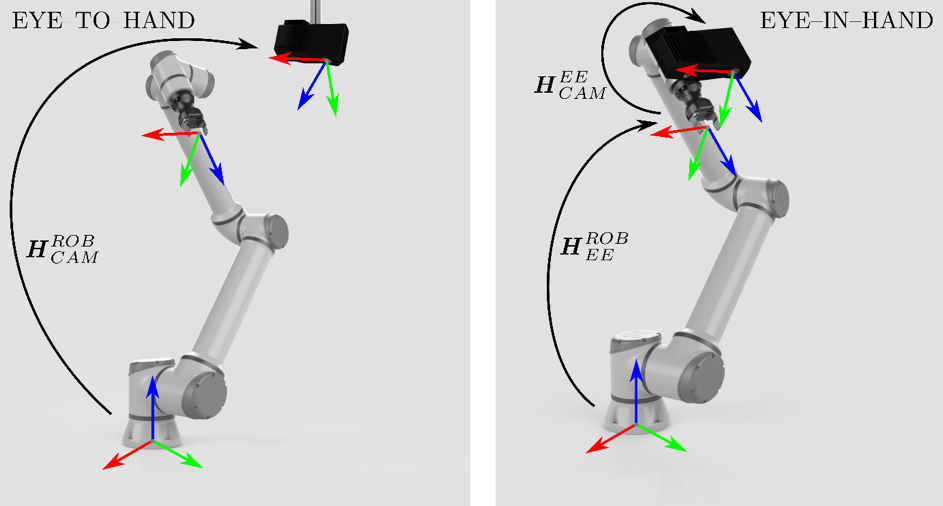
\includegraphics[width=0.9\linewidth]{images/chapter2Images/eye_to_in_hand.png}
	\caption{Comparison between the eye-in-hand and eye-to-hand configurations used in hand-eye calibration. In the eye-in-hand setup, the camera is mounted on the robot end-effector and moves together with the manipulator, whereas in the eye-to-hand setup the camera remains fixed in the environment and observes the robot workspace externally. The unknown transformation $\mathbf{X}$ changes depending on the selected configuration.}
	\label{fig:eye_in_hand_vs_eye_to_hand}
\end{figure}


In this case the motion matrices become:

\begin{equation}
    \mathbf{A}_i = \left({}^B_E\mathbf{T}_j\right)^{-1} {}^B_E\mathbf{T}_k,
    \qquad
    \mathbf{B}_i = \left({}^C_O\mathbf{T}_j\right)^{-1} {}^C_O\mathbf{T}_k
    \label{eq:AB_eth}
\end{equation}

\noindent and the same $\mathbf{AX} = \mathbf{XB}$ structure of
equation~\eqref{eq:axxb} is preserved \cite{horaud1995hand,
enebuse2021comparative}. This configuration is commonly used in inspection
systems where the camera observes the robot workspace from a fixed vantage point.

% -- Figure [IMG-8] --
% (see figure suggestions at the end of this section)

% ---------------------------------------------------------------
\subsection{Solution Methods}
\label{subsec:hec_methods}
% ---------------------------------------------------------------

Several methods have been proposed in the literature to solve
equation~\eqref{eq:axxb}. They can be broadly classified as follows.

\paragraph{Two-stage closed-form methods.}
The earliest approaches \cite{shiu1989calibration, tsai1989new} solve the
rotation sub-problem~\eqref{eq:rot_subproblem} first, then recover the
translation from the linear system~\eqref{eq:trans_subproblem}. While
computationally efficient, these methods suffer from error propagation from the
rotation stage to the translation stage.

\paragraph{Simultaneous rotation--translation methods.}
Horaud and Dornaika \cite{horaud1995hand} showed that estimating rotation and translation
within a unified formulation can provide
improved robustness to measurement noise than the two-stage
decomposition. 



\paragraph{Dual quaternion method.}
Daniilidis \cite{daniilidis1999hand} reformulated the problem using dual
quaternions, representing each transformation as:

\begin{equation}
    \hat{\mathbf{q}} = \mathbf{q}_r + \varepsilon\, \mathbf{q}_d,
    \qquad \varepsilon^2 = 0
    \label{eq:dual_quat}
\end{equation}

\noindent where $\mathbf{q}_r$ is the real part encoding rotation and
$\mathbf{q}_d$ is the dual part encoding translation. This formulation allows
rotation and translation to be recovered simultaneously from a single SVD
decomposition, avoiding the numerical coupling issues of two-stage methods.


% ---------------------------------------------------------------
\subsection{Observability Conditions and Degenerate Motions}
\label{subsec:observability}
% ---------------------------------------------------------------

A critical aspect of hand-eye calibration is the \textit{observability} of the
system. Not all robot motions contribute equally to constraining the solution
$\mathbf{X}$ \cite{strobl2006optimal, shiu1989calibration}.

For the rotation component to be uniquely determined from
equation~\eqref{eq:rot_subproblem}, the rotation axes of the collected motions
$\mathbf{A}_i$ must not all be parallel. Formally, the rotation sub-problem is
uniquely solvable if and only if there exist at least two motion pairs whose
rotation axes are not collinear \cite{park1994robot}. For the translation
component~\eqref{eq:trans_subproblem} to be uniquely solvable, at least one
motion must contain a non-zero rotational component.

The following robot motions lead to \textit{degenerate configurations} that
must be avoided during data acquisition:

\begin{itemize}
    \item \textbf{Pure translations} without any rotation: the rotation
    sub-problem~\eqref{eq:rot_subproblem} provides no information, since
    $\mathbf{R}_{A_i} = \mathbf{I}$.

    \item \textbf{Rotations around a single fixed axis}: all rotation axes are
    parallel, and the rotation $\mathbf{R}_X$ is determined only up to a rotation
    around that axis.

    \item \textbf{Very small or near-zero motions}: the motion matrices
    $\mathbf{A}_i \approx \mathbf{I}$ carry little geometric information and
    amplify the effect of measurement noise.
\end{itemize}

In practice, a diverse and well-distributed set of robot poses should be collected
during data acquisition, ensuring that the end-effector rotates around multiple
non-parallel axes by sufficiently large angles \cite{strobl2006optimal}. The
quality of the pose set directly determines the conditioning of the calibration
problem and, consequently, the accuracy of the estimated transformation
$\mathbf{X}$.

\bigskip
\noindent\textit{Suggested figure for this section:}
\begin{itemize}
    \item \textbf{[IMG-8]} Eye-in-hand vs.\ eye-to-hand configuration diagram.
    Show two side-by-side schematics of a robot arm. On the left (eye-in-hand):
    the camera is mounted on the end-effector, the target is on the table, and
    $\mathbf{X} = {}^E_C\mathbf{T}$ is labelled between the end-effector and
    camera frames. On the right (eye-to-hand): the camera is on a stand, the
    target is on the end-effector, and $\mathbf{X} = {}^C_B\mathbf{T}$ is
    labelled between the camera and robot base frames. This figure is expected
    in every hand-eye calibration thesis and immediately clarifies the two
    configurations for the reader. I can generate it in TikZ if you want.
\end{itemize}




% ---------------------------------------------------------
% Hand-Eye Calibration Pipeline Flowchart
% ---------------------------------------------------------

\begin{figure}[htbp]
	\centering
	
	\begin{tikzpicture}[
		node distance=1.2cm,
		every node/.style={font=\small},
		block/.style={
			rectangle,
			rounded corners,
			draw=black,
			thick,
			align=center,
			minimum width=5cm,
			minimum height=0.9cm
		},
		arrow/.style={
			thick,
			-{Latex[length=3mm]}
		}
		]
		
		\node[block] (robot) {Robot poses acquisition};
		
		\node[block, below=of robot] (images) {Image acquisition};
		
		\node[block, below=of images] (detection) {ChArUco target detection};
		
		\node[block, below=of detection] (pnp) {PnP pose estimation};
		
		\node[block, below=of pnp] (motion) {Motion pair construction\\ $(\mathbf{A}_i,\mathbf{B}_i)$};
		
		\node[block, below=of motion] (solver) {Hand-eye calibration solver};
		
		\node[block, below=of solver] (validation) {Calibration validation};
		
		\draw[arrow] (robot) -- (images);
		\draw[arrow] (images) -- (detection);
		\draw[arrow] (detection) -- (pnp);
		\draw[arrow] (pnp) -- (motion);
		\draw[arrow] (motion) -- (solver);
		\draw[arrow] (solver) -- (validation);
		
	\end{tikzpicture}
	
	\caption{Typical hand-eye calibration pipeline adopted in robot vision systems. The workflow starts from synchronized robot poses and image acquisition, followed by target detection, camera pose estimation, motion pair construction, calibration solving, and final validation.}
	\label{fig:handeye_pipeline}
	
\end{figure}




\section{Related Work}

Hand-eye calibration is the problem of estimating the rigid transformation between a robot end-effector (the \emph{hand}) and a camera or sensor rigidly attached to it (the \emph{eye}). In the eye-in-hand setting, a static calibration target is observed from multiple robot poses: robot kinematics provide the pose of the gripper with respect to the robot base, while pose estimation on the calibration target provides the pose of the target with respect to the camera. The resulting formulation is commonly written as an equation of the form
\begin{equation}
\mathbf{A}_{ij}\mathbf{X} = \mathbf{X}\mathbf{B}_{ij},
\label{eq:axxb}
\end{equation}
where \(\mathbf{X}\) is the unknown hand-eye transformation and \(\mathbf{A}_{ij}\), \(\mathbf{B}_{ij}\) are relative motions computed from two different observations \(i\) and \(j\). A common convention is
\begin{equation}
\mathbf{A}_{ij} = \left({}^{b}\mathbf{T}_{g,j}\right)^{-1} {}^{b}\mathbf{T}_{g,i},
\qquad
\mathbf{B}_{ij} = {}^{c}\mathbf{T}_{t,j}\left({}^{c}\mathbf{T}_{t,i}\right)^{-1},
\end{equation}
with \({}^{b}\mathbf{T}_{g}\) the gripper pose in the robot base frame and \({}^{c}\mathbf{T}_{t}\) the calibration target pose in the camera frame. OpenCV's \texttt{calibrateHandEye} follows this classical eye-in-hand formulation and provides several established solvers, including Tsai, Park, Horaud, Andreff, and Daniilidis. \cite{OpenCVHandEye}

\subsection*{Classical methods}

Early solutions to hand-eye calibration focused on closed-form or semi-closed-form estimation strategies. A landmark contribution is the method of Tsai and Lenz, which separates the estimation of rotation and translation and first solves the rotational part before recovering the translation. Their formulation is computationally efficient and has become a standard baseline in robotics and vision calibration. \cite{Tsai1989}

Park and Martin derived a solution on the Euclidean group using Lie-theoretic tools, providing a closed-form exact solution and a least-squares solution in the presence of noise. Their formulation is elegant from a geometric point of view because it works directly on the rigid-motion structure of \(SE(3)\) rather than treating rotation and translation as unrelated quantities. \cite{ParkMartin1994}

Horaud and Dornaika proposed a unified framework that treats the hand-eye problem with a nonlinear optimization approach. In their formulation, rotation and translation can be estimated simultaneously, which makes the method particularly attractive when the measurement noise is non-negligible. A more recent stability analysis also reports that the simultaneous nonlinear approach is among the most robust with respect to noise and measurement errors. \cite{HoraudDornaika1995,HoraudDornaika2023}

For the rotational subproblem, the hand-eye equation can be decomposed as
\begin{equation}
\mathbf{R}_{A_{ij}}\mathbf{R}_X = \mathbf{R}_X \mathbf{R}_{B_{ij}},
\end{equation}
while the translational component becomes
\begin{equation}
\left(\mathbf{R}_{A_{ij}} - \mathbf{I}\right)\mathbf{t}_X =
\mathbf{R}_X\mathbf{t}_{B_{ij}} - \mathbf{t}_{A_{ij}}.
\label{eq:translation}
\end{equation}
This separable structure is the reason why several classical algorithms estimate rotation first and then solve translation by least squares. \cite{Tsai1989,ParkMartin1994}

\subsection*{Optimization-based approaches}

More recent approaches formulate hand-eye calibration as a nonlinear least-squares problem over several motion pairs. A typical objective is
\begin{equation}
\min_{\mathbf{X}\in SE(3)} \sum_{(i,j)} \left\|
\log\!\left(\mathbf{A}_{ij}\mathbf{X}\mathbf{B}_{ij}^{-1}\mathbf{X}^{-1}\right)
\right\|^2,
\label{eq:nonlinear_objective}
\end{equation}
where \(\log(\cdot)\) denotes the matrix logarithm on \(SE(3)\). This type of formulation directly minimizes the geometric inconsistency of the calibration equations and is often used as a refinement step after a closed-form initialization. The advantage is improved accuracy; the drawback is a higher computational cost and a stronger dependence on a good starting point. \cite{HoraudDornaika2023,Enebuse2022}

\subsection*{Dual quaternion methods}

Another important family of methods is based on dual quaternions, which represent rigid transformations in a compact algebraic form by combining rotation and translation in a single object. A dual quaternion can be written as
\begin{equation}
\hat{\mathbf{q}} = \mathbf{q}_r + \varepsilon \mathbf{q}_d,
\end{equation}
where \(\mathbf{q}_r\) is the unit quaternion associated with rotation, \(\mathbf{q}_d\) encodes translation, and \(\varepsilon\) is the dual unit with \(\varepsilon^2 = 0\). Daniilidis and Bayro-Corrochano showed that this representation allows the hand-eye problem to be solved in a unified way, often via a linear system and singular value decomposition. \cite{Daniilidis1996}

Dual quaternion formulations are appealing because they avoid splitting rotation and translation into two separate steps. This can lead to compact expressions and numerically elegant solvers, although the implementation is usually less immediate than for matrix-based methods. \cite{Daniilidis1996}

\subsection*{Practical implementations and experimental considerations}

In practical industrial pipelines, hand-eye calibration is commonly implemented using software libraries rather than from scratch. OpenCV, for example, exposes a dedicated \texttt{calibrateHandEye} function and supports multiple classical algorithms, which makes it a convenient reference implementation for comparing different calibration strategies. \cite{OpenCVHandEye}

The accuracy of the final result depends not only on the chosen algorithm but also on the quality of the input poses, the calibration target detection, and the robot motion design. Recent experimental studies report that rotation noise, translation noise, and the motion range used during acquisition can all have a significant impact on calibration accuracy. In particular, separated and simultaneous methods may react differently to the same motion pattern, which motivates careful data collection and method selection in real applications. \cite{Enebuse2022}

In this work, these considerations motivate a practical calibration pipeline based on established solvers, explicit validation of the estimated poses, and attention to the acquisition geometry. Particular emphasis is placed on the integration of the calibration procedure within an industrial vision workflow, where the reliability of pose estimation and the interoperability of software components are both critical. \cite{OpenCVHandEye,Enebuse2022}


